\scanpage{12}
\mspage{4}
\margin{
($n$ odd)

\uline{Proposition} There exist liftings $\widetilde\rho,\widetilde\sigma$ of
$\rho,\sigma$ such that we have $\widetilde\rho^{n}=\widetilde\sigma^{2}$
\deleted{\unsure{$\rho$}}, and the two \unsure{sides} are then of the form
$\widetilde\omega^{\nu}$,
\inserted{\unsure{one of the}}
\deleted{\unsure{for all}},
$\nu$ \unsure{\uline{well-defined quantity}|\deleted{well-defined quantity}}
\unsure{modulo} $2n$ (\unsure{independently} of the choices of the liftings
$\widetilde\rho,\widetilde\sigma$)
and $\nu\equiv\dfrac{\unsure{n^2+1}}{2}$
\deleted{\unsure{$\mathbb Z$}}, \unsure{or} :
\[
\nu\ \mathrm{mod}\ 2n\ \in
\left\{\unsure{(}-\frac{n-1}{2},\frac{n+1}{2}\unsure{)}\right\}
\]
and $\nu$ is odd.
Which implies that there exists \unsure{a} $\nu_0$ \unsure{unique} in
$\left\{-\dfrac{n-1}{2},\dfrac{n+1}{2}\right\}$ that is
$\equiv\nu\ (2n)$.
For $\nu$ fixed, $\widetilde\rho,\widetilde\sigma$ are \unsure{uniquely} \unsure{determined}.
\unsure{Thus we find|This provides} \unsure{presentation}
\[
\widetilde\Pi_n^D=
\left\{\widetilde\rho,\widetilde\sigma,\widetilde\omega\ \middle|\
\widetilde\omega\text{ central},\
\widetilde\rho^n=\widetilde\sigma^2=\widetilde\omega^{\unsure{\nu_0|\nu}}\right\}.
\]
}

\diagram{\begin{tikzcd}[ampersand replacement=\&,row sep=1.5em,column sep=4em]
1 \arrow[d] \& \& 0 \arrow[d]
\\
\mathbb Z\widetilde\omega \arrow[d]
\& \widetilde\omega=(1,2n)
\& \mathbb Z \arrow[d,"2n"]
\\
\widetilde\Pi_n^D \arrow[d] \arrow[rr] \& \& \mathbb Z \arrow[d]
\\
\Pi_n^D=\{\rho,\sigma\mid\rho^n=\sigma^2=1\}
\arrow[d] \arrow[rr,Rightarrow]
\& \& (\Pi_n^D)_{\mathrm{ab}}\simeq\mathbb Z/2n\mathbb Z
\\
1 \& \&
\begin{gathered}
\rho\longmapsto(n+1\ \mathrm{mod}\ 2n)=(1-n\ \mathrm{mod}\ 2n)\\
\sigma\longmapsto n\ \mathrm{mod}\ 2n
\end{gathered}
\end{tikzcd}}

\[
\begin{aligned}
\widetilde\rho_0&=(\rho,n+1)\\
\widetilde\sigma_0&=(\sigma,n)
\end{aligned}
\qquad
\begin{aligned}
\widetilde\rho_0^n&=(\overbrace{\rho^n}^{1},n(n+1))
 =\deleted{\unsure{\widetilde\omega^{n+1}}}\\
\widetilde\sigma_0^2&=(\underbrace{\sigma^2}_{1},2n)
\end{aligned}
\]
\[
\widetilde\rho_0^n/\widetilde\sigma_0^2
=(1,n(n-1))=\widetilde\omega^{\alpha}
\]
\[
\alpha=\frac{n-1}{2}\qquad
(\alpha=1\text{ if }n=3\unsure{!|?})
\]
\[
\bigl(\widetilde\rho_0\widetilde\omega^{\unsure{\beta}}\bigr)^n
=\bigl(\widetilde\sigma_0\widetilde\omega^{\gamma}\bigr)^2
\qquad\text{i.e.}\quad
\widetilde\rho_0^n\widetilde\sigma_0^{-2}
=\widetilde\omega^{\deleted{\unsure{n\beta-2\gamma}}\inserted{2\gamma-n\beta}}
\]
\[
\alpha+1
\]
\[
\deleted{\unsure{n}}\qquad
2\gamma-n\beta=\alpha=\frac{n-1}{2}
\]
\[
\deleted{4\gamma-2n\beta=}
\]
\[
\widetilde\rho\overset{\text{definition}}=
\widetilde\rho_0\widetilde\omega^{\overbrace{\unsure{\beta}}^{\alpha}}
=\left(\rho,n+1+
\underbrace{2n\overbrace{\frac{n-1}{2}}^{\beta=\alpha}}_{n(n-1)}\right)
=(\rho,n^2+1)
\]
\[
\widetilde\sigma\overset{\text{definition}}=
\widetilde\sigma_0\widetilde\omega^{\gamma}
=\left(\sigma,
\underbrace{
\deleted{\unsure{4}}n+
\underbrace{2n\underbrace{\gamma}_{\frac{(n-1)(n+1)}{4}=\frac{n^2-1}{4}}}
_{\frac{n^3-n}{2}}}_{\frac{n^3+n}{2}}
\right)
=\left(\sigma,\deleted{\unsure{\frac{n^3-n}{2}}}\inserted{\frac{n^3+n}{2}}\right)
\]
\[
\begin{array}{|l}
(\alpha+1).2-1.n=1\\
\underbrace{\alpha(\alpha+1)}_{\gamma}.2-
\underbrace{\alpha}_{\beta}.n=\alpha
\end{array}
\qquad\gamma=
\]
\margin{
\[
\begin{array}{|l}
\widetilde\rho=\widetilde\rho_0\widetilde\omega^{2x}\\
\widetilde\sigma=\widetilde\sigma_0\widetilde\omega^{nx}\\[1em]
x=
\end{array}
\]
}
\[
\begin{aligned}
\widetilde\rho_0^n&=(1,n^3+n)=
\widetilde\omega^{\overbrace{\frac{n^2+1}{2}}^{\nu}}\\
\widetilde\sigma_0^2&=(1,n^3+n)=\widetilde\omega^{\frac{n^2+1}{2}}
\end{aligned}
\]
\margin{11}

\scanpage{13}
% not manuscript: fin d'une lettre manuscrite signée Escofier, au sujet du recrutement en Statistiques et Analyse des données; écriture distincte de celle des calculs.

\scanpage{14}
\mspage{4bis}
\[
\begin{aligned}
\widetilde\rho^{\unsure{*|n}}&=(\rho,n^2+1)\\
\widetilde\sigma^{\unsure{2|*}}&=\left(\sigma,\frac{n^3+n}{2}\right)
\end{aligned}
\qquad
\bigl(\widetilde\rho\widetilde\omega^{\beta}\bigr)^n
=\bigl(\widetilde\sigma\widetilde\omega^{\gamma}\bigr)^2
\]
\[
\widetilde\rho^n\simeq\widetilde\sigma^{\unsure{2|n}}
=\widetilde\omega^{\frac{n^2+1}{2}}
\qquad
\begin{gathered}
\Updownarrow\\
\widetilde\omega^\nu\widetilde\omega^{\beta n}
=\widetilde\omega^\nu\widetilde\omega^{\gamma2}
\end{gathered}
\]
\[
\beta n=2\gamma
\]
\[
n^2-n\qquad\frac{n-1}{2}\qquad\deleted{\unsure{\beta=}}
\]
\diagram{\begin{tikzcd}[ampersand replacement=\&,row sep=0.5em,column sep=2em]
\mathbb Z^2\arrow[r]\&\mathbb Z\\
(\beta,\gamma)\&
\end{tikzcd}}
\[
\begin{aligned}
\beta&=2x\\
\gamma&=nx
\end{aligned}
\qquad
\beta n=2\gamma=(2n)x
\]
\[
\nu+\uline{2nx}
\]
\[
\frac{n^2+1}{2}\ \mathrm{mod}\ 2n
\qquad\qquad
\frac{n^2+1}{2}.\ \mathrm{mod}\ 2n
\]
\[
13\ \mathrm{mod}\ 10\ /\ 3
\qquad\qquad
\unsure{n=3}\quad5\ \mathrm{mod}\ 6=
\]
\[
n=2\alpha+1
\]
\[
\frac{n^2+1}{2}
=\frac{4\alpha^2+4\alpha+2}{2}
=\underbrace{2\alpha^2+2\alpha+1}_{
\begin{array}{ll}
(4\alpha+2)\dfrac{\alpha}{2}+\alpha+1&\text{if }\alpha\text{ even}\\
\underbrace{(4\alpha+2)\dfrac{\alpha+1}{2}}_{2\alpha^2+3\alpha+1}
\unsure{-}\alpha&\text{if }\alpha\text{ odd}
\end{array}}
\quad\mathrm{mod}\quad4\alpha+2
\]
\[
\frac{n^2+1}{2}\equiv\alpha+1=\frac{n+1}{2}
\quad(2n)\qquad\text{if }\alpha\text{ even}
\]
\[
\frac{n^2+1}{2}\equiv-\alpha=\frac{1-n}{2}
\quad(2n)\qquad\text{if }\alpha\text{ odd}
\]
\[
\rho^n=\widetilde\sigma^2=\widetilde\omega^{\frac{n+1}{2}}
\quad\text{if }\frac{n+1}{2}\text{ is odd i.e. }\alpha=\frac{n-1}{2}\text{ even}
\]
\[
\widetilde\rho^{\unsure{n}}=\widetilde\sigma^2
=\widetilde\omega^{-\frac{n-1}{2}}
\quad\text{if }\frac{n-1}{2}\text{ is odd}
\]
so we \unsure{find} \unsure{a}
\[
\widetilde\rho^{\unsure{n}}=\widetilde\sigma^2=\widetilde\omega^\nu
\]
where
\[
\nu\in\left\{-\frac{n-1}{2},\deleted{\unsure{2}}\frac{n+1}{2}\right\},
\quad\nu\text{ odd}
\]
which suffices to \unsure{characterize} $\unsure{\nu}$.
\margin{13}

\scanpage{15}
\deleted{
\diagram{\begin{tikzcd}[ampersand replacement=\&,column sep=2em]
\Pi_{03}^{D}\arrow[r]
\&\underbrace{\mathbb Z/6\mathbb Z\mathbin{\times}_{\mathbb Z/2\mathbb Z}\mathbb D_3}_{18}
=\left\{\nu,\unsure{g''|g'}\in\mathbb Z/6\mathbb Z\times\mathbb D_3\ \middle|\
\unsure{\mathrm{sg}^{+}|\mathrm{sg}^{t}}(g)\equiv\nu\ (2)\right\}
\end{tikzcd}}

\[
\overset{\deleted{\unsure{\mathrm{ext}}}}{\Pi_{0,3\,\mathrm{ab}}}
\simeq\mathbb Z^3/\mathbb Z
\]
\[
\Pi_{0,3\,\mathrm{ab}}\otimes_{\mathbb Z}\mathbb F_3
=\mathbb F_3^3/\mathbb F_3
\supset\deleted{\unsure{V}}
\bigl(\mathbb F_3^{3\,\unsure{0|1}}\bigr)/\mathbb F_3
\]
\[
\rho_0\quad\rho_1\quad\rho_\infty\quad
\left\{\begin{array}{l}
\rho_0\rho_1^{-1},\quad\rho_1\rho_\infty^{-1},\quad
\rho_\infty\rho_0^{-1},\quad\rho_0^3\\
\deleted{[\rho_0,\rho_1]}\quad
\deleted{[\rho_1,\rho_\infty]}\quad
\deleted{[\rho_\infty,\rho_0]}
\end{array}\right.
\]

\[
\underbrace{\mathrm S\ell(2,\mathbb Z/6\mathbb Z)/\{\pm1\}}
_{\substack{\deleted{\text{of order}}\\72}}
\simeq
\bigl(\underbrace{\mathrm S\ell(2,\unsure{\mathbb Z/2\mathbb Z})}_{6}
\times\underbrace{\mathrm S\ell(2,\mathbb Z/3\mathbb Z)}_{24}\bigr)/_{\pm1}
\]
\[
p(p-1)(p+1)
\]
\[
\left\{\rho,\sigma\ \middle|\
\rho^3=\sigma^2=\deleted{\unsure{\omega\rho_0}}(\sigma\rho)^6=1,\quad
\overset{\inserted{(\sigma\rho)^2=\rho\bigl((\sigma\rho)^2\bigr)}}
{\sigma\rho\sigma\rho=\rho\sigma\rho\sigma}
\right\}
\]

\[
\begin{aligned}
\rho_0&=\sigma\rho\sigma\rho\\
\rho_1&=\rho\sigma\rho\sigma
\end{aligned}
\]
\deleted{\[
\begin{aligned}
\relax[\rho_0,\rho_1]
&=\sigma\rho\sigma\rho\rho\sigma\rho\sigma\rho^{-1}\sigma
\underbrace{\rho^{\unsure{-1}}\deleted{\sigma}\deleted{\sigma}\rho^{\unsure{-1}}}_{\rho^{-2}}
\sigma\rho^{\unsure{-1}}\\
&=\sigma\rho\sigma\rho^2\sigma\rho\sigma\rho^{-1}\sigma\rho^{-2}\sigma\rho^{-1}
\end{aligned}
\]}
\[
\sigma\rho\sigma\rho\sigma\rho^{-1}\sigma\rho^{-1}
\]
\[
\varepsilon_0=\sigma\rho
\]
}

\margin{\[
\sigma\rho\sigma\rho=1
\]
\[
\unsure{.}\,2\quad4
\]
\diagram{\begin{tikzcd}[ampersand replacement=\&,column sep=1.7em,row sep=1.4em]
\rho\arrow[r,mapsto]\&\begin{gathered}2\ \mathrm{mod}\ 6\\4\ \mathrm{mod}\ 6\end{gathered}\\
\unsure{\sigma}\arrow[r,no head]\&3\ \mathrm{mod}\ 6
\end{tikzcd}}}

\[
% the last glyph is inverted: it stands in the orientation of the printed text, not of the handwriting
\rho_0\qquad\rho_1\qquad\rho_\infty\qquad\unsure{5|\varepsilon}
\]
\[
\rho_0=\deleted{\unsure{\rho\sigma}}\sigma\rho\sigma^{-1}\rho
=(\sigma\rho)^2\omega
\]
\margin{14}

% Printed non-manuscript administrative substrate, upside down relative to
% the mathematical handwriting; transcribed here in its own reading order.
principle and the procedures for these subdivisions are left to the initiative of the
Committees. However, the proportions fixed in article 2 will have to be respected
in a subcommittee.

\uline{ARTICLE 5.-}

Under the chairmanship of the President of the U.S.T.L., a committee composed
of all the Vice-Presidents and of the Vice-President of the Scientific Council, is
in particular charged with determining the number of seats to be filled in each
of the expanded Committees of specialists, and, in general,with
giving its opinion on all the problems that might arise in connection
with their establishment and their operation.

\uline{ARTICLE 6.-}

All provisions of the internal regulations contrary to the present text
are repealed.

\scanpage{16}
\mspage{5}

$M_{1,1}\simeq (U_{0,3},\mathbb D'_3)$, where $\mathbb D'_3$ is defined as the fiber product

\diagram{\begin{tikzcd}[ampersand replacement=\&,row sep=large,column sep=large]
\mathbb D_3=\unsure{\mathfrak S_3|\mathfrak G_3} \arrow[r,"\mathrm{can}"] \& \mathbb Z/2\mathbb Z \\
\mathbb D'_3 \arrow[u] \arrow[r] \& \mathbb Z/4\mathbb Z \arrow[u,"\mathrm{can}"']
\end{tikzcd}}

\margin{\uuline{to be checked}\quad\uline{OK}}

so $\mathbb D'_3$ is an extension (\unsure{nontrivial|quite trivial}) of $\mathbb D_3$ by $\mathbb Z/2\mathbb Z$ ; \deleted{\unsure{when}} we let $\mathbb D'_3$ act on $U_{0,3}$ via $\mathbb D_3$, so \unsure{with triviality} of the element $\omega$ of order $2$ of the \unsure{kernel} of $\unsure{\mathbb D'_2|\mathbb D'_3}\to\unsure{\mathbb D_2|\mathbb D_3}$.

We thus have

\diagram{\begin{tikzcd}[ampersand replacement=\&,column sep=small,row sep=small]
\mathcal T_{11} \arrow[r,phantom,"\simeq"] \arrow[d,phantom,"\simeq"{sloped}] \& \Pi_1\overbrace{(U_{0,3},\mathbb D'_3;P_+)}^{\Pi_{0,3}^{\mathbb D'_3}} \\
\mathrm S\ell(2,\mathbb Z) \&
\end{tikzcd}}

\margin{depends on the choice of a point of the Poincaré half-plane \unsure{above} $P_+$, \unsure{we will take|or take} $\zeta=\exp(2i\pi/6)$\quad$\uline{\unsure{a}}$}

and thus

\margin{$\unsure{\Pi_\rho|\Pi_0}\qquad\unsure{\Pi_{0,3}}$}

\figure{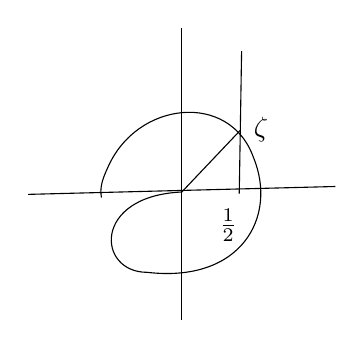
\begin{tikzpicture}[x=1cm,y=1cm]
\draw (-1.95,-.03)--(1.95,.07);
\draw (0,-1.62)--(0,2.08);
\draw (0,0) .. controls (-1.14,-.05) and (-1.08,-1.02) .. (-.44,-1.02) .. controls (.76,-1.16) and (1.22,-.31) .. (.91,.44) .. controls (.61,1.28) and (-.57,1.16) .. (-.94,.31) .. controls (-1.02,.14) and (-1.04,.04) .. (-1.02,-.07);
\draw (.73,-.02)--(.76,1.79);
\draw (0,0)--(.74,.78);
\node[right] at (.79,.79) {$\zeta$};
\node[below] at (.59,-.09) {$\frac12$};
\end{tikzpicture}}

\diagram{\begin{tikzcd}[ampersand replacement=\&,row sep=large,column sep=large]
\Pi_{0,3}^{\mathbb D'} \arrow[r] \arrow[d] \& \Pi_{0,3}^{\mathbb D}=\{\rho,\sigma\mid\rho^3=\sigma^2=1\} \arrow[d,Rightarrow] \\
\deleted{\unsure{\mathbb Z/4\mathbb Z}}\,\inserted{\unsure{\mathbb D'_3}} \arrow[r] \arrow[d] \arrow[ur,phantom,"\unsure{\mathrm{cart}}"{description}] \& \deleted{\unsure{\mathbb Z/2\mathbb Z}}\,\inserted{\unsure{\mathbb D_3}} \arrow[d] \\
\mathbb Z/4\mathbb Z \arrow[r,no head] \arrow[ur,phantom,"\unsure{\mathrm{cart}}"{description}] \& \mathbb Z/2\mathbb Z
\end{tikzcd}}

\margin{$\deleted{\rho\mapsto0,\quad\sigma\mapsto1}$\par
$\rho\mapsto0$\par
$\sigma\mapsto1$}

\margin{\unsure{We lift} $\rho,\sigma$ to $\deleted{\unsure{\rho,\sigma}}\ \rho',\sigma'$\par
$\rho'=(\rho,2),\quad\sigma'=(\sigma,\deleted{\unsure{2}}\inserted{3})$\par
\unsure{we have}
$\rho'^{\,6}=\sigma'^{\,4}=1,$\par
$\rho'^{\,3}=\sigma'^{\,2}=(\underbrace{1,2\bmod4}_{\omega})$.}

\margin{We then easily verify that\par
$\mathrm S\ell(2,\mathbb Z)\simeq\{\rho',\sigma'\mid \unsure{\rho'^{\,6}=\sigma'^{\,4}=1},\ \unsure{\rho'^{\,3}=\sigma'^{\,2}}\}$.}

\margin{\figure{\begin{tikzpicture}[x=1cm,y=1cm]
\draw[->] (2.92,3.25) .. controls (2.82,2.34) and (1.35,2.38) .. (1.05,1.46) .. controls (.92,1.12) and (.86,.77) .. (.71,.58);
\draw (0.05,2.24) .. controls (.42,1.64) and (.29,1.03) .. (.21,.96) .. controls (.12,.88) and (.24,.73) .. (.35,.68);
\draw (.59,.98) .. controls (.43,.46) and (.48,.12) .. (.35,-.02) .. controls (.62,.12) and (.63,-.29) .. (.67,-.72);
\end{tikzpicture}}}

Thus $\Pi_{0,3}^{\mathbb D'}\simeq\mathrm S\ell(2,\mathbb Z)$ \unsure{appears} as an extension of $\Pi_{0,3}^{\mathbb D}$ by $\mathbb Z/2\mathbb Z$, inverse image \deleted{\unsure{of}} the extension \inserted{$\mathbb D'_3$} of $\mathbb D_3$ by $\mathbb Z/2\mathbb Z$, or of the extension $\mathbb Z/4\mathbb Z$ of $\mathbb Z/2\mathbb Z$ by $\mathbb Z/2\mathbb Z$, via $\Pi_{0,3}^{\mathbb D}\to\mathbb D_3$ \unsure{resp.} composite $\Pi_{0,3}^{\mathbb D}\to\deleted{\unsure{\mathbb D_3}}\mathbb Z/2\mathbb Z$. \unsure{It is} an extension of $\mathbb D'_3$ by a \unsure{group} $\simeq\Pi_{0,3}$, \unsure{with basis} $\rho_0,\rho_1,\rho_\infty$ \unsure{---}

\margin{15}